\chapter{Metodologia}\label{cap:metod}
\section{Software de Rastreio e Decodificação}\label{sec:software}
\begin{figure}[h]
    \centering
    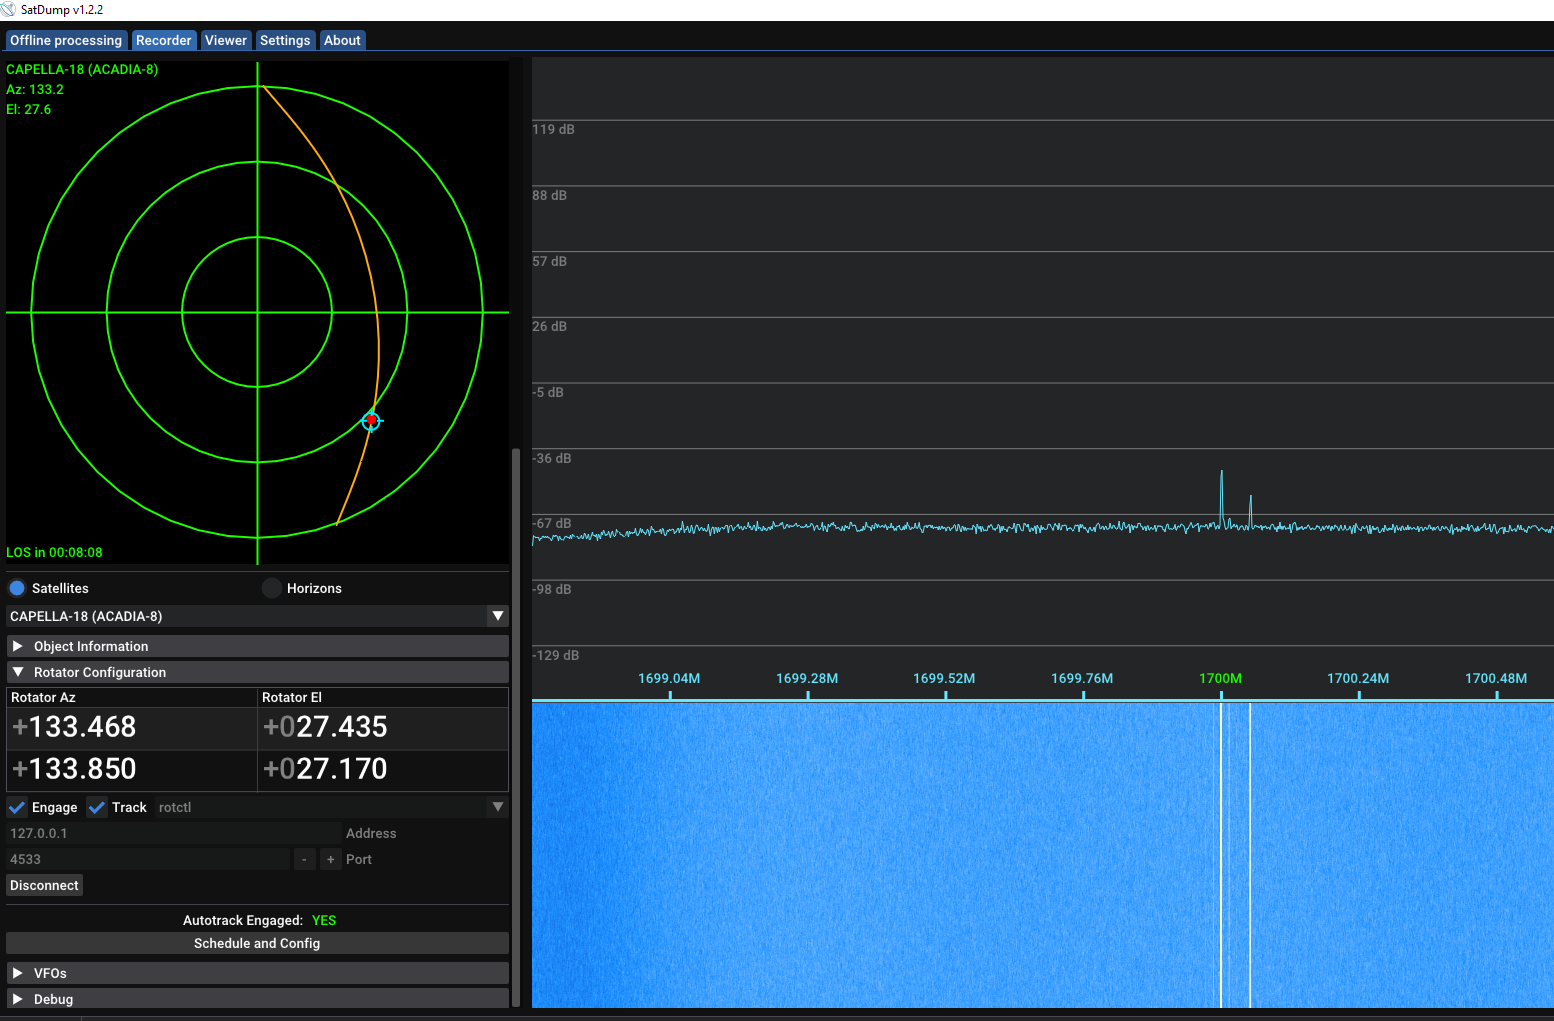
\includegraphics[width=0.8\textwidth]{figs/satdump_example.png}
    \caption{Interface do software SatDump}
    \caption*{Fonte: Autor(2026)}
    \label{fig:satdump}
\end{figure}
O aplicativo de rastreio de satélites principal do trabalho será o SatDump.
Esse programa será utilizado porque ele possui um conglomerado de ferramentas para permitir o rastreio de satélites e a decodificação dos sinais recebidos pela antena da estação de solo.
Na figura \ref{fig:satdump}, é possível observar a interface do Software. O software está dividido em duas partes principais: a painel de controle/rastreio (à esquerda) e o analisador de espectro/cachoeira RF (à direita).

Na região esquerda, existe uma roda polar no topo, que indica algumas informações sobre o satélite rasteado. O texto acima da roda indica o satélite que está sendo rastreado (no caso, o CAPELLA-18), além de suas informações de azimute e elevação.
Abaixo do texto, está a roda polar de fato. A roda polar é uma representação bidimensional de 360° de toda a abóbada celeste visível a partir da localização da estação em solo. O centro do círculo, onde há a intersecção dos eixos, representa o Zênite (elevação de $90^{\circ}$), enquanto os círculos concêntricos indicam as elevações intermediárias de $0^{\circ}$, $30^{\circ}$ e $60^{\circ}$ (do mais externo para o mais interno).
A cruz interna representa a direção cardeal, ou seja, em qual direção do horizonte a antena deve apontar. A seção superior da cruz indica $0/360^{\circ}$, representando o Norte, e o ângulo de azimute é crescente no sentido horário. Desta forma, a linha direita indica $90^{\circ}$ (Leste), a linha inferior indica $180^{\circ}$ (Sul), e a linha esquerda indica $270^{\circ}$ (Oeste).
A linha amarela representa todo o arco que o satélite faz durante essa passagem. O ponto vermelho indica a posição real do satélite. O ícone de mira azul indica a posição que foi passada ao rotor da antena, enquanto o círculo azul representa a posição que o rotor acusa estar.
Mais abaixo há um texto com a informação de tempo estimado até ocorrer a LOS (Loss of signal, ou perda de sinal) do satélite quando este se encontrar abaixo do horizonte.
Na seção de nome "Rotator Configuration" (configuração de rotor), esta área está destinada à conexão do programa com o rotor. Os números de azimute e elevação de da linha superior é a posição teórica onde o satélite está, calculada com base nas informações de órbita e a posição da estação de solo.
A linha inferior indica a posição real de apontamento da antena indicada pelo rotor. Abaixo disso, há a configuração do servidor de controle dos rotores, na qual estão configurados o endereço de IP e a porta para a comunicação. Além disso, existem as opções de "Engage" (engajar), que inicia a conexão com servidor, e "Track" (rastrear), que envia posições atualizadas ao mecanismo de apontamento.

A região direita é dedicada ao processamento e à representação visual do sinal de radiofrequência (RF) recebido pelo aplicativo. Este painel fornece diagnóstico em tempo real da qualidade do enlace de comunicação e é composto por dois elementos gráficos fundamentais alinhados no domínio da frequência: o Analisador de Espectro e o Exibidor em Cachoeira (Waterfall).
O gráfico superior exibe a densidade de potência do sinal capturado em função da frequência, calculada por meio da Transformada Rápida de Fourier (FFT). Seu eixo vertical representa a amplitude (em \text{dB}, decibel) do sinal recebido para cada frequência, enquanto o eixo horizontal indica a frequência em $\text{MHz}$.
O gráfico inferior é conhecido como visualizador em cachoeira representa a variação observada no gráfico acima em função do tempo (eixo y). Esse visualizador é atualizado com as informações mais novas sendo inseridas em cima e as mais antigas "deslizando" para regiões mais abaixo. Esse gráfico é mapeado por cores, nos quais cores próximas ao azul indicam uma intensidade baixa, enquanto cores próximas ao vermelho indicam uma maior intensidade de sinal recebida.
Em geral, essa interface é utilizada para garantir a estabilidade da transmissão durante a passagem, além de permitir observar variações na largura do sinal ou desvios na frequência central da linha ao longo do rastreio.

\section{Motores de Passo}\label{sec:motor_passo}
O sistema de controle da antena será baseado em um pedestal convencional
controlado por dois parâmetros ortogonais principais, sendo estes: azimute e elevação.
Para efetuar o controle desses fatores em uma antena, serão necessários dois motores que atuarão modificando
os ângulos mencionados anteriormente. Como discutido na seção \ref{sec:ground_tracking}, o controle do azimute será feito por 360 graus, enquanto o
controle de elevação atuará somente em 90 graus. Desta maneira, o ângulo de visada total do mecanismo
será dado por uma meia-esfera superior. Essa geometria é considerada suficiente para a detecção e o rastreio de qualquer satélite necessário pela estação de solo.

Os motores de passo utilizados no trabalho são de classe NEMA (National Electrical Manufacturers Association, Associação Nacional de Fabricantes de Equipamentos Elétricos), que padroniza as dimensões e as características de motores em geral. O modelo selecionado é o motor de passo 17HS4401, da classe NEMA 17.
Ele possui ângulo de passo de $1.8^{\circ}\pm5\%$, torque de $4,2\text{kgf}\cdot\text{cm}$, e corrente por fase de $1,5A$.
\begin{figure}[h]
    \centering
    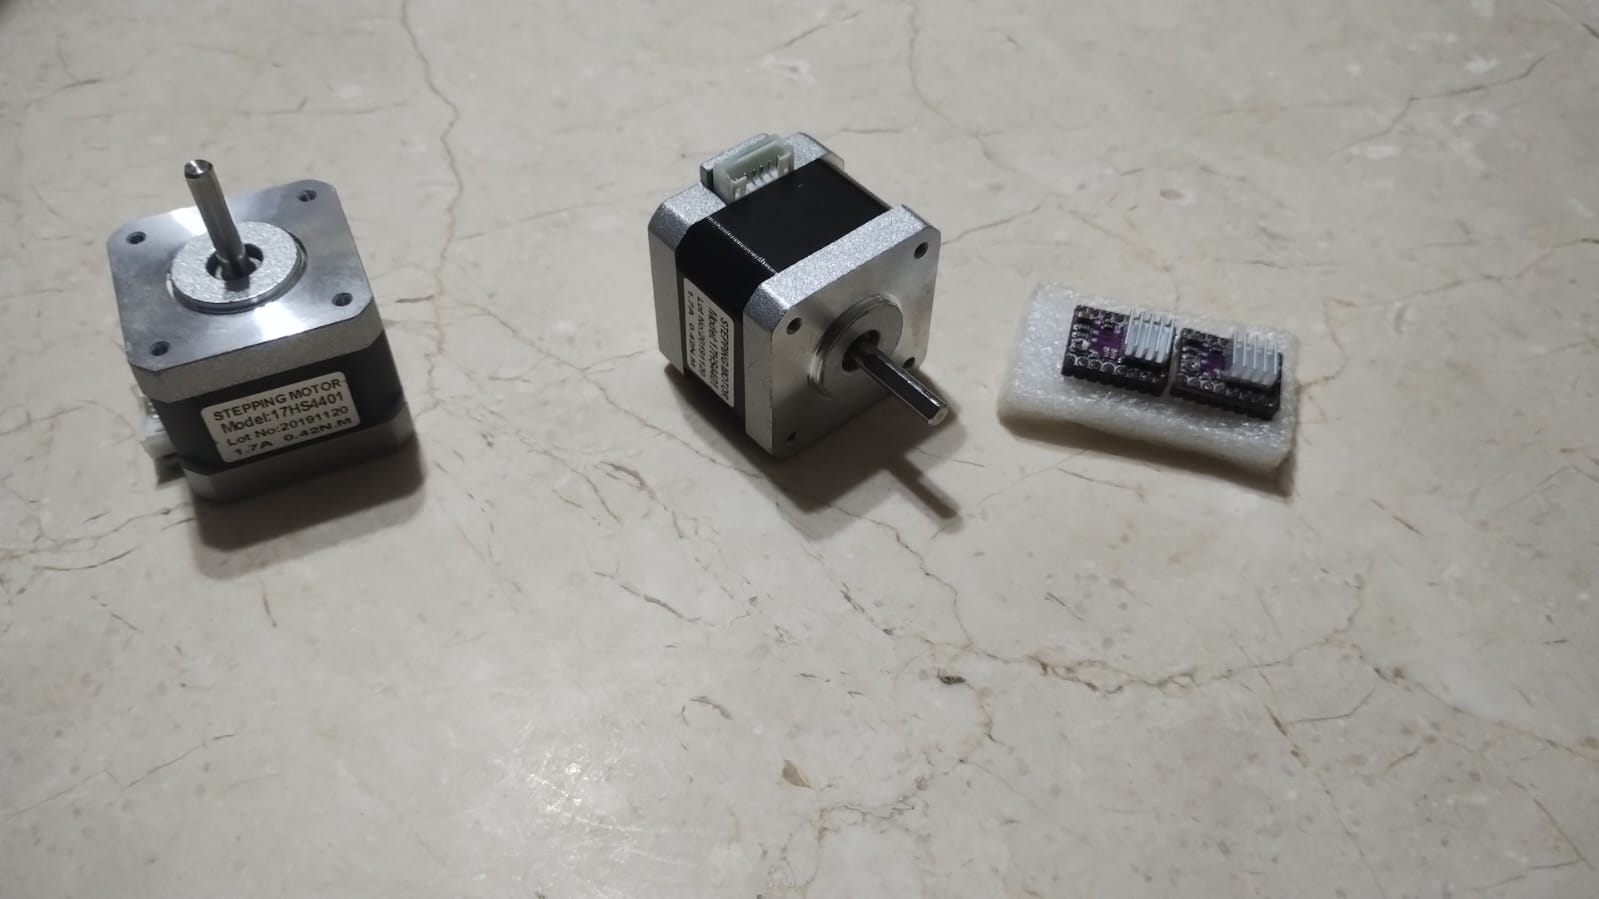
\includegraphics[width=0.8\textwidth]{figs/motores_drivers.jpeg}
    \caption{Motores 17HS4401 e drivers DRV8825}
    \caption*{Fonte: Autor(2026)}
    \label{fig:motores_drivers}
\end{figure}

Para o acionamento dos motores, serão utilizados drivers dedicados DRV8825, configurados para conseguirem atingir a resolução de $1/32$ passo, permitindo elevar a resolução angular teórica de acionamento dos motores para $0,05625^\circ$ por micropasso.
A calibração da posição inicial (homing) das eixos de azimute e elevação será realizada por meio de sensores ópticos, que serão desenvolvidos a partir de LDRs e LEDs. O controlador fará uma varredura para verificar quando o LDR receberá a maior intensidade luminosa. Esse valor máximo indicará o zero do azimute e da elevação.
O acoplamento entre o eixo dos motores e a estrutura da antena será feito utilizando um sistema de redução por correias GT2 de relação 2:1, fazendo com que a resolução real na estrutura seja metade da resolução angular desenvolvida pelo motor.

\begin{figure}[h]
    \centering
    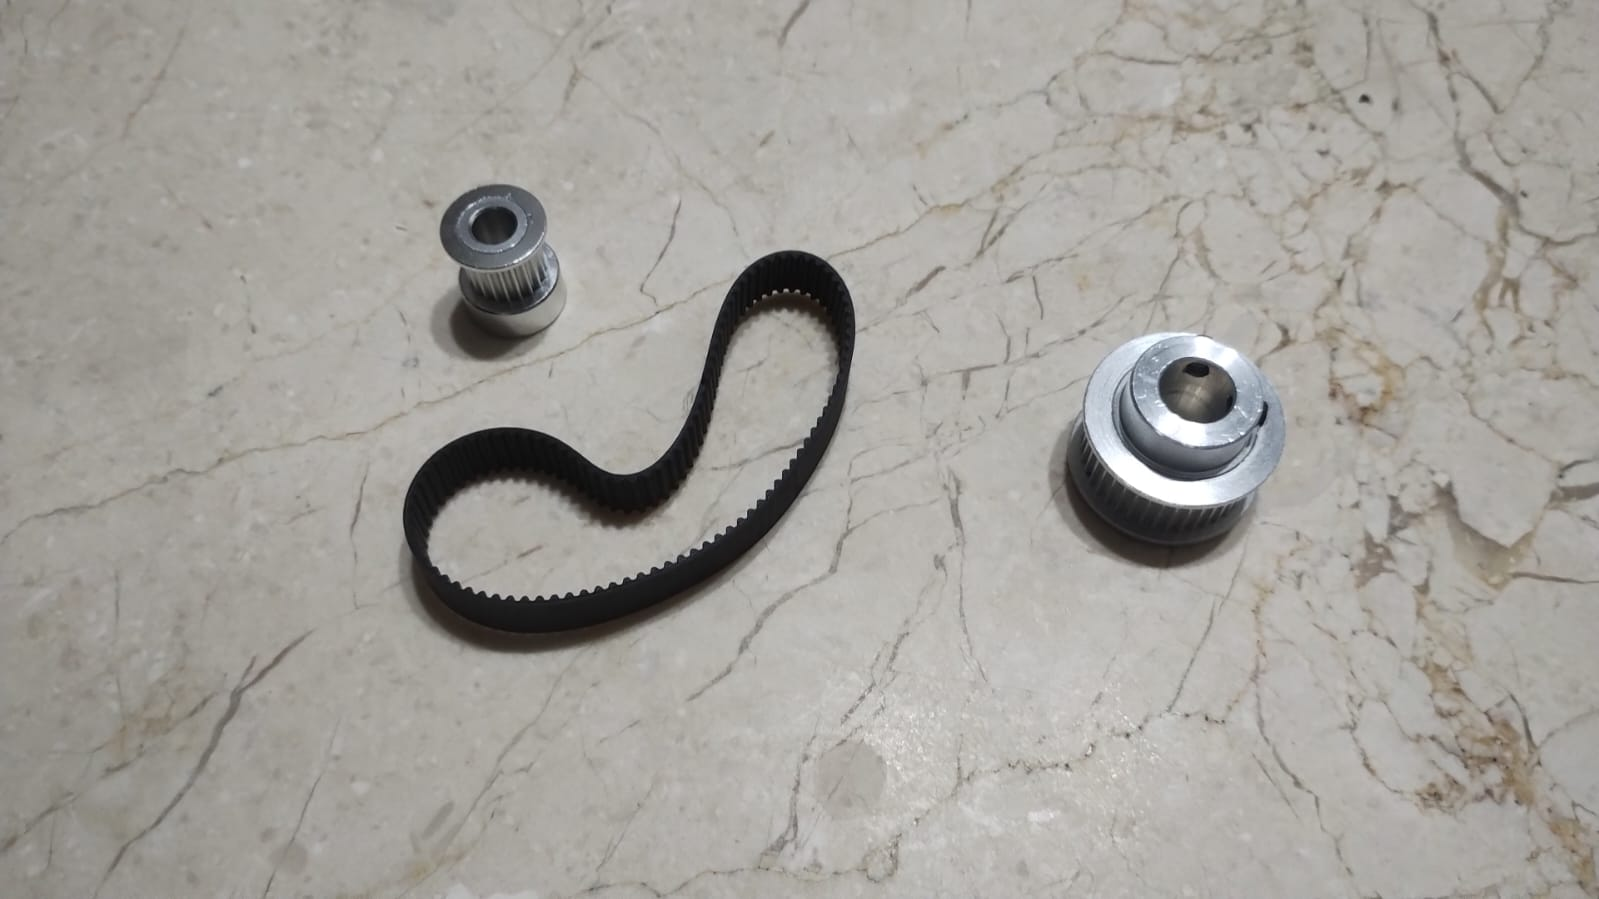
\includegraphics[width=0.8\textwidth]{figs/polias_cinto.jpeg}
    \caption{Polias GT2 com 20 e 40 dentes, além de cinto de 200mm}
    \caption*{Fonte: Autor(2026)}
    \label{fig:polias_cinto}
\end{figure}

\section{Sistema de Comunicação}\label{sec:sistema_comunicacao}
Para o recebimento do sinal de satélite, será utilizando um rádio definido por software (Software Defined Radio, ou SDR), de modelo RTL-SDR V4. Esse dispositivo é capaz de ser programado via software para sintonizar com diversas frequências sem modificação de hardware, tornando-o extremamente versátil para receber comunicação de diversos satélites.
O modelo em questão é capaz de operar em frequências de \SI{500}{\kilo\hertz} a \SI{1766}{\mega\hertz}. Além disso, há um circuito Bias-Tee interno ativável por software, que é capaz de fornecer uma tensão contínua de 4,5 V no conector SMA para alimentação de pré-amplificadores localizados na linha de transmissão utilizando o mesmo cabo coaxial por onde o sinal é recebido.

Devido à extrema atenuação sofrida pelos sinais emitidos pelos satélites ao se propagarem através da atmosfera até a antena de recepção, será utilizado um módulo pré-amplificador e filtrador Nooelec SAWBird+ GOES.
O módulo é composto por dois estágios de amplificação de baixo ruído (LNA) em cascata com um filtro de Onda Acústica de Superfície (SAW) intercalado. Esses compontentes são responsáveis por tratar, filtrar e amplificar os sinais recebidos pela antena.
O conjunto apresenta frequência central em aproximadamente \SI{1688}{\mega\hertz}, com banda passante ajustada para a recepção de \SI{1694,1}{\mega\hertz} e ganho típico de 35 dB, reduzindo interferências de sinais fora da faixa de interesse e compensando as perdas de transmissão.

Todo o sistema será montado dentro do cabo da antena e haverá um cabo extensor USB de \SI{2}{\meter} para realizar a conexão com o computador. O sistema de recepção está representado na figura \ref{fig:sistema_coms}.

\begin{figure}[h]
    \centering
    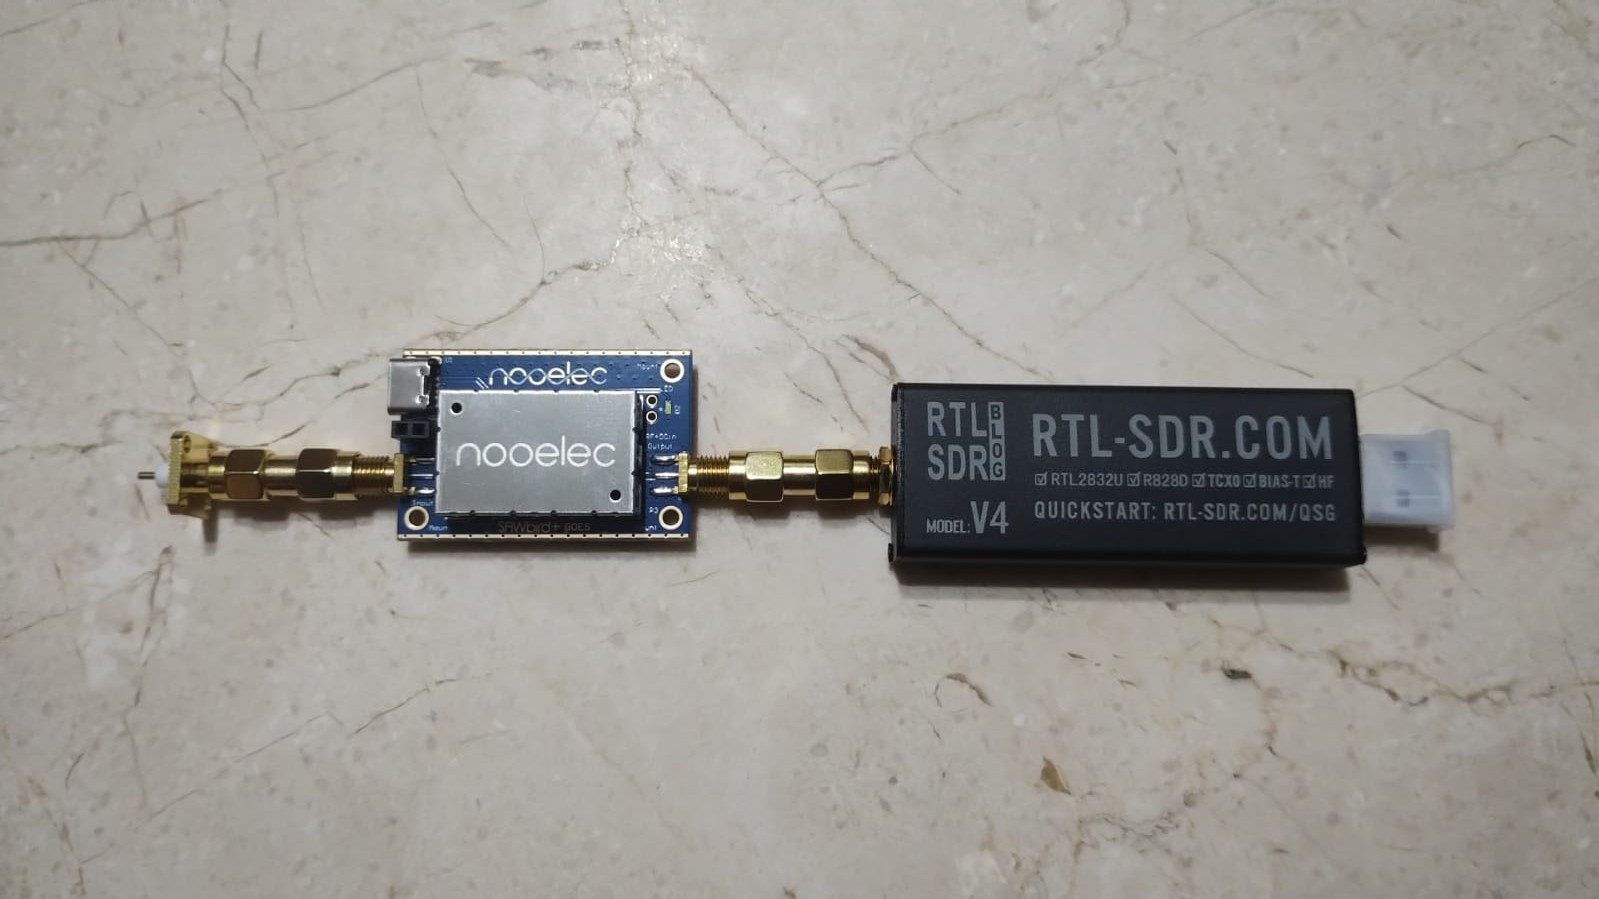
\includegraphics[width=0.8\textwidth]{figs/sistema_comunicacao.jpeg}
    \caption{Sistema de comunicação com ponto de alimentação da antena (dourado) à esquerda, filtro Nooelec (azul) ao centro e SDR (preto) à direita}
    \caption*{Fonte: Autor(2026)}
    \label{fig:sistema_coms}
\end{figure}

\section{Antena}\label{sec:antena}

\begin{figure}[h]
    \centering
    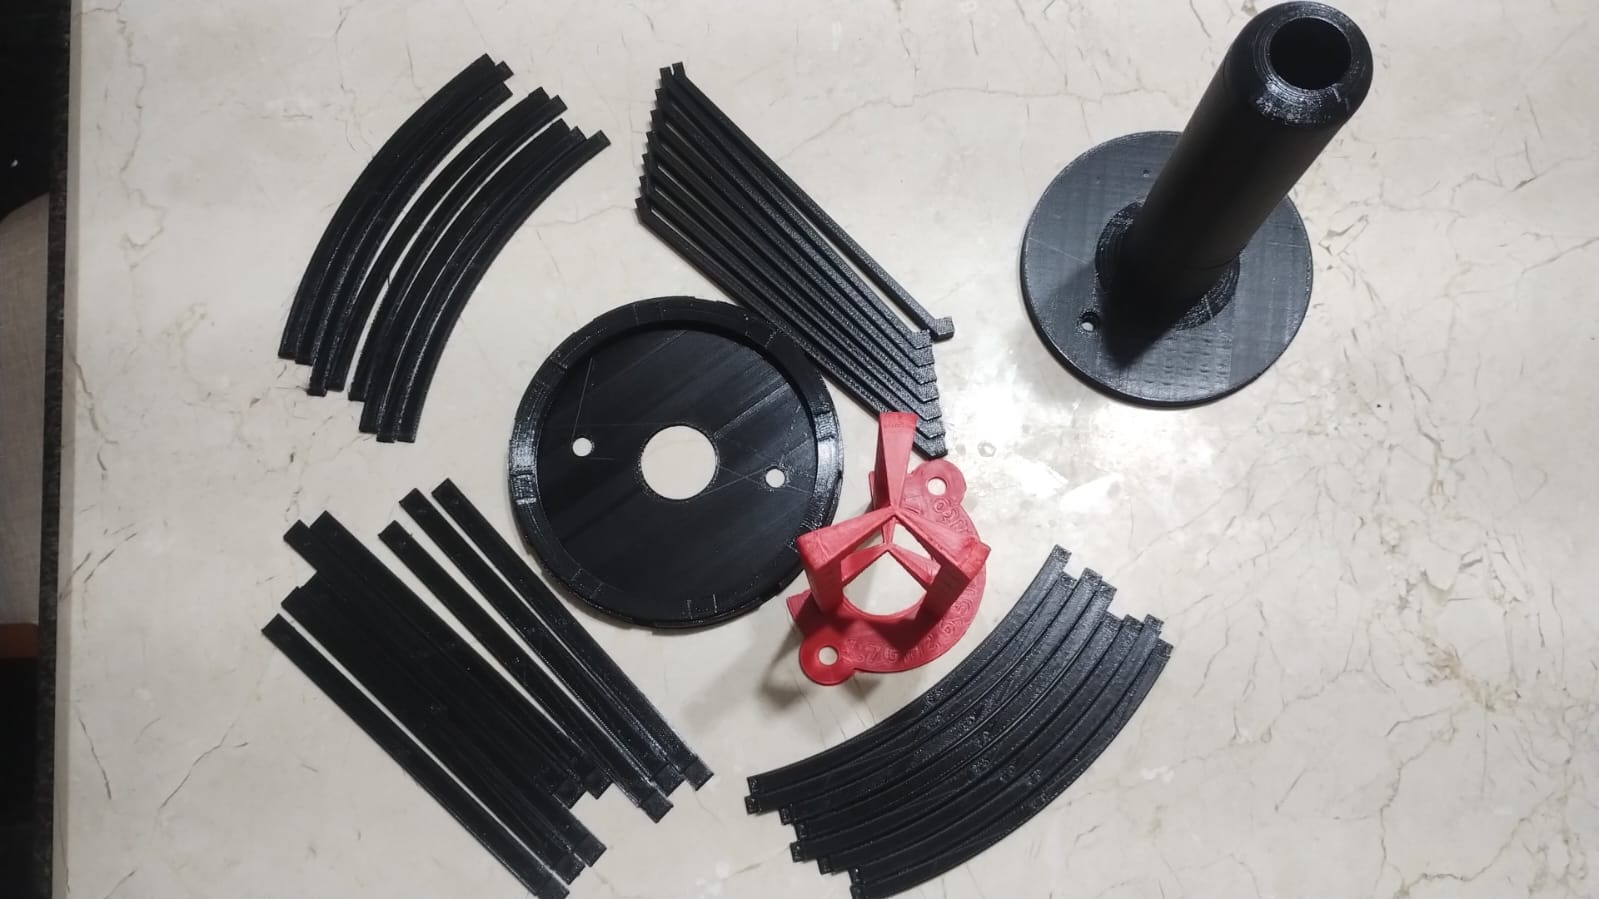
\includegraphics[width=0.8\textwidth]{figs/antena_peças.jpeg}
    \caption{Sistema de comunicação com ponto de alimentação da antena (dourado) à esquerda, filtro Nooelec (azul) ao centro e SDR (preto) à direita}
    \caption*{Fonte: Autor(2026)}
    \label{fig:pecas_antena}
\end{figure}

A antena apresentada no projeto de \cite{tonito2024} é uma Antena Helicone projetada especificamente para a recepção de sinais de alta resolução de satélites meteorológicos na faixa de 1,7 GHz, desenvolvida para a captura de imagens enviadas no modo HRPT (High Resolution Picture Transmission).
Este modelo combina a simplicidade construtiva com características eletromagnéticas de alto ganho e alta diretividade, sendo ideal tanto para uso  montado no sistema de rastreio automatizado desenvolvido nessa tese.
A antena helicone é uma variação da antena helicoidal no modo axial combinada com um plano Terra (ground plane) levemente cônico.

Satélites que transmitem em HRPT operam com Polarização Circular (normalmente RHCP — Right-Hand Circular Polarization).
Uma antena com hélice helicoidal garante o casamento de polarização correto com a onda incidente, evitando perdas severas de sinal por descasamento de polarização (Polarization Mismatch Loss), comuns em antenas de polarização linear em movimento.
Quando a circunferência de cada volta da hélice é próxima ao comprimento de onda da frequência central ($\mathbf{C \approx \lambda}$), a antena passa a emitir e receber no modo axial.
Nesse regime, o feixe de radiação principal fica concentrado na direção do eixo da hélice $$\lambda = \frac{c}{f} = \frac{3 \times 10^8\text{ m/s}}{1,7 \times 10^9\text{ Hz}} \approx 176,4\text{ mm}$$.
Com o diâmetro da hélice do projeto fixado em torno de $56\text{ mm}$, a circunferência $C = \pi \cdot d = \pi \cdot 56\text{ mm} \approx 175,9\text{ mm}$, o que corresponde precisamente ao regime do modo axial.

\section{Sistema Embarcado}\label{sec:sistema_embarcado}
Com o intuito de manter o servidor de controle do rotor embarcado no pedestal, será utilizado um microcontrolador de modelo de desenvolvimento ESP32 WROOM-32.
Além disso, para manter uma interface gráfica disponível para fácil entendimento de seu operador, o sistema contará com um display de LCD (Liquid Crystal Display, ou tela de cristal líquido) para mostrar telemetria de apontamento e informações de conexão.
\begin{figure}[h]
    \centering
    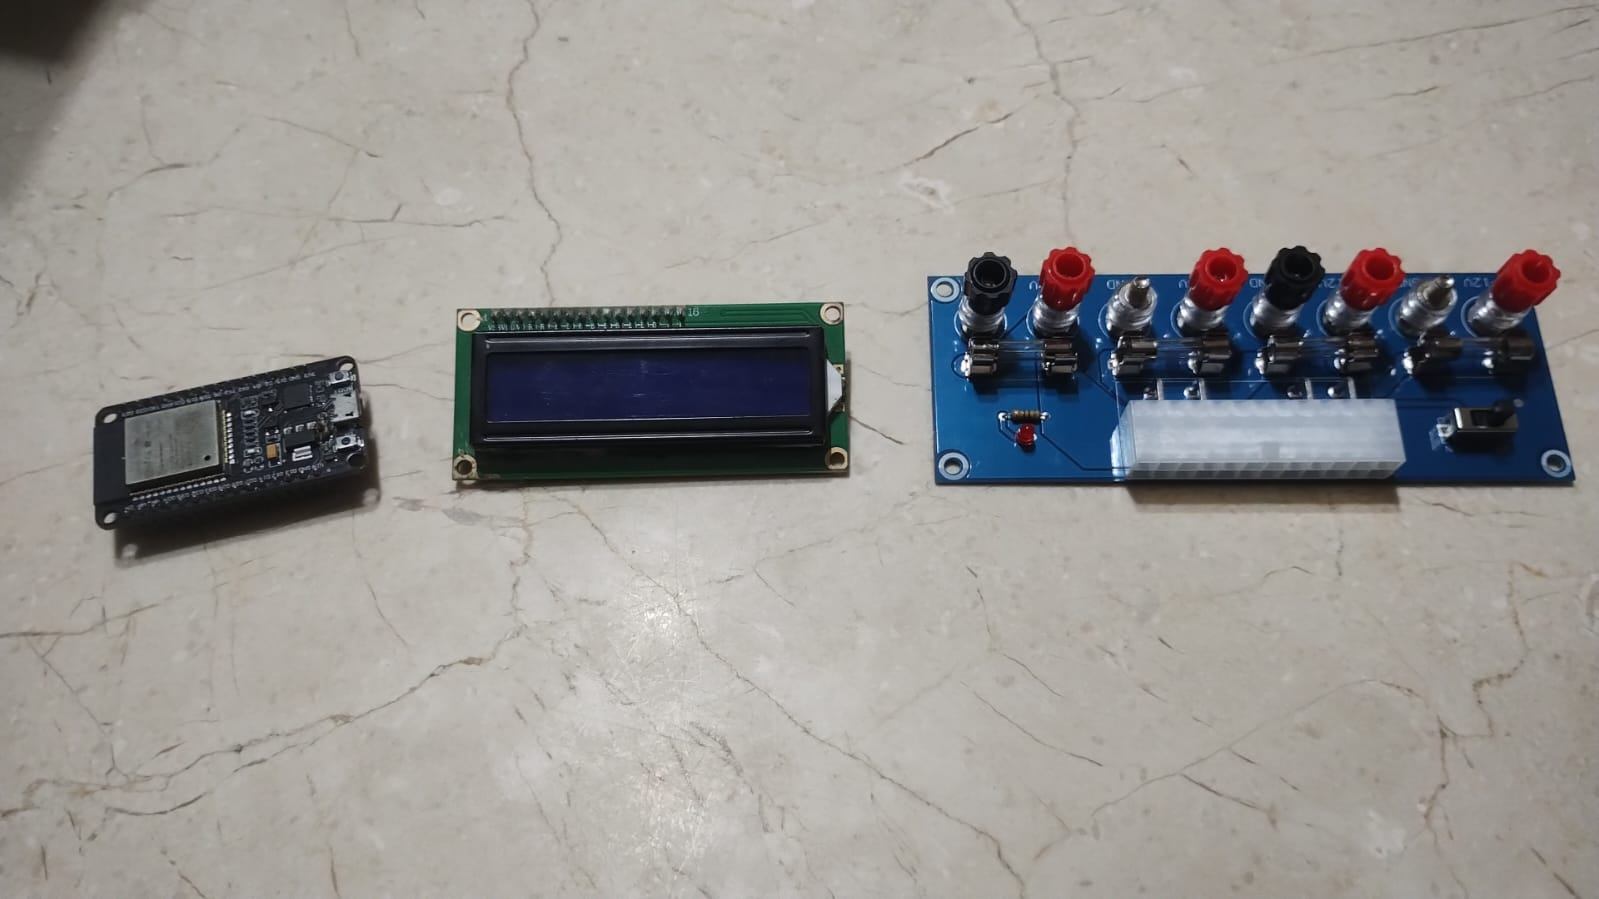
\includegraphics[width=0.8\textwidth]{figs/embarcados_peças.jpeg}
    \caption{Componentes parte do sistema embarcado, sendo o ESP32 (esquerda), display de LCD (centro), e adaptador de fonte 24 pinos de computador (direita).}
    \caption*{Fonte: Autor(2026)}
    \label{fig:embarcados_pecas}
\end{figure}

A arquitetura do sistema foi desenvolvida aproveitando a estrutura dual-core do ESP32, permitindo o processamento paralelo de tarefas por meio do FreeRTOS (Real-Time Operating System).
Esse sistema operacional em tempo real e de código aberto permite a divisão do programa em tarefas independentes, alocadas em cada um dos núcleos do microcontrolador.
A carga de trabalho do projeto está dividida da seguinte maneira: o núcleo 0 (vindo da contagem a partir da base 0) é responsável por toda a interface de comunicação, sendo essas o controle do servidor TCP e a interface com o LCD, enquando o núcleo 1 é responsável pelo controle do motor e do filtro $\alpha-\beta-\gamma$ embarcado.
Dessa forma, essa arquitetura garante um processador esteja exclusivamente destinado ao controle das malhas do motor, evitando que interferências ou latências de comunicação afetem a estabilidade e a precisão do rotor.

\begin{figure}[h]
    \centering
    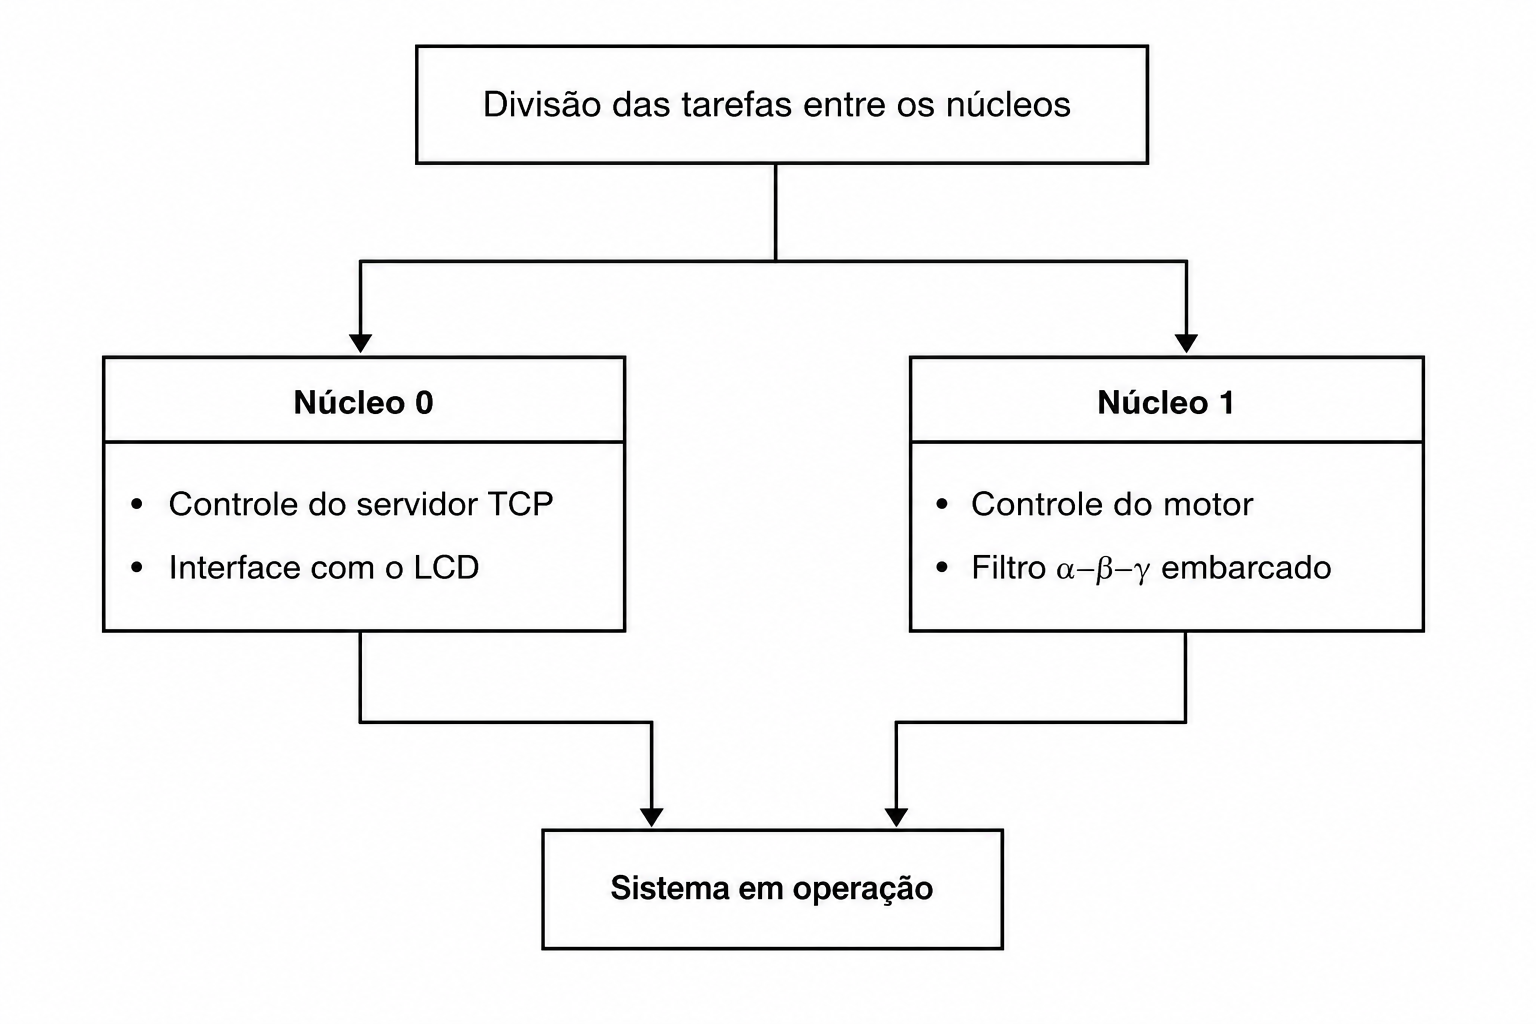
\includegraphics[width=0.8\textwidth]{figs/divisao_tarefas_nucleos_esp.png}
    \caption{Diagrama de divisão de tarefas entre os núcleos do microcontrolador.}
    \caption*{Fonte: Autor(2026)}
    \label{fig:divisao_tarefas_esp}
\end{figure}

\section{Implementação do Filtro Preditor}\label{sec:implementacao_filtro}
Para determinar os parâmetros do filtro preditor que será embarcado no processador, foram feitos alguns testes a partir de um servidor dummy (simulado) em um computador. Esse servidor era encarregado de receber todos os comandos enviados pelo software e catalogar as posições esperadas em diversos rastreios.
As capturas foram realizadas através de diversos dias, garantindo uma grande variação nas órbitas obtidas.
A partir desses dados, foi desenvolvido um algoritmo capaz de utilizar os valores dentro do limite de estabilidade discutido na seção \ref{sec:estimation} para encontrar o filtro cujos parâmetros geram o menor Erro Quadrático Médio (EQM ou MSE, na sigla em inglês).
Esse algoritmo altera os parâmetros alfa, beta e gama de acordo com um certo passo determinado e expõe todos os filtros aos mesmos dados, garantindo que a entrada não tenha um viés e os filtros estejam expostos às mesmas condições.
Com o Erro Quadrático Médio calculado para cada parâmetro, é possível estipular valores para o $\alpha$, $\beta$ e $\gamma$ que obtenha o melhor resultado preditivo de forma generalizada.
Deste modo, esses parâmetros calibrados foram embarcados na arquitetura do sistema apresentada na Seção \ref{sec:sistema_embarcado}.

\section{Controle de Velocidade e posição do Motor de Passo}\label{sec:controle_motor_passo}
A posição da estrutura é determinada de forma incremental a partir da posição inicial do motor, da relação de transmissão do sistema e da contagem dos pulsos emitidos pelo driver.
Embora o driver DRV8825 suporte frequências de pulso elevadas (de até aproximadamente 250 kHz), a resposta dinâmica dos motores de passo NEMA é mais restrita, limitando sua operação contínua a frequências na faixa de 1000 Hz.
Portanto, o controlador deve gerar sinal em uma frequência compatível com o motor, aproveitando a capacidade de micropasso (microstepping) do driver para aumentar a resolução e suavizar o deslocamento.
A partir dos valores de posição, velocidade e aceleração estimados pelo filtro $\alpha-\beta-\gamma$, o sistema calcula posições intermediárias preditas e determina as frequências de passo necessárias para realizar tal ação.
Essa interpolação reduz trancos na estrutura e garante um alinhamento mais estável e contínuo com o satélite.
Assim, com base na velocidade estimada pelo filtro, o controlador calcula a frequência de pulsos enviada ao DRV8825 para os eixos de azimute e elevação.
Para otimizar o tempo de processamento, é possível empregar equações simplificadas ou tabelas de consulta (lookup tables) pré-calculadas, ajustando a frequência e a resolução de passo necessárias para atingir a velocidade desejada em cada eixo.
